% to run: lualatex ttZ_EFT.tex
\RequirePackage{luatex85}
\documentclass[tikz, border=10pt]{standalone}

\usepackage[compat=1.1.0]{tikz-feynman}

\newcommand{\Ptop}{\ensuremath{\mathrm{t}}}
\newcommand{\Pg}{\ensuremath{\mathrm{g}}}
\newcommand{\Pq}{\ensuremath{\mathrm{q}}}
\newcommand{\PH}{\ensuremath{\mathrm{H}}}
\newcommand{\PW}{\ensuremath{\mathrm{W}}}
\newcommand{\PZ}{\ensuremath{\mathrm{Z}}}

\begin{document}
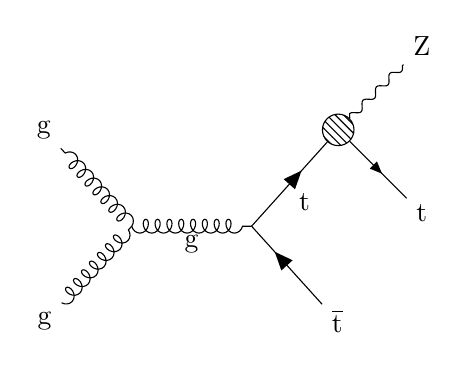
\begin{tikzpicture}
  \begin{feynman}
    \diagram [horizontal=a to b] {
      i1 [particle=\(\Pg\)] -- [gluon] a -- [gluon] i2 [particle=\(\Pg\)],
      a -- [gluon, edge label'=\(\Pg\)] b,
      c [blob, minimum size=0.4cm] -- [anti fermion, edge label=\(\Ptop\)] b -- [anti fermion] f2 [particle=\(\overline \Ptop\)],
    };

    \vertex [above right=of c] (d) {\(\PZ\)};
    \vertex [below right=of c] (e) {\(\Ptop\)};

    \diagram* [arrow size=1pt] {
      (d) -- [boson] (c) -- [fermion] (e);
    };
  \end{feynman}
\end{tikzpicture}
\end{document}
